% THIS DOCUMENT IS FOLLOWS THE VOLERE TEMPLATE BY Suzanne Robertson and James Robertson
% ONLY THE SECTION HEADINGS ARE PROVIDED
%
% Initial draft from https://github.com/Dieblich/volere
%
% Risks are removed because they are covered by the Hazard Analysis
\documentclass[12pt]{article}

\usepackage{booktabs}
\usepackage{tabularx}
\usepackage{hyperref}
\usepackage{multicol}
\usepackage[dvipsnames]{xcolor}
\usepackage{enumitem}
\usepackage{tcolorbox}
\usepackage{array}

\hypersetup{
    bookmarks=true,         % show bookmarks bar?
      colorlinks=true,      % false: boxed links; true: colored links
    linkcolor=red,          % color of internal links (change box color with linkbordercolor)
    citecolor=green,        % color of links to bibliography
    filecolor=magenta,      % color of file links
    urlcolor=cyan           % color of external links
}

\newenvironment{myreq}[1]{%
\setlist[description]{font=\normalfont\color{darkgray}}%
\begin{tcolorbox}[colframe=black,colback=white, sharp corners, boxrule=1pt]%
\bfseries\color{blue}%
\begin{description}#1}%
{\end{description}\end{tcolorbox}}

\newcommand{\threeinline}[3]{\begin{multicols}{3}#1 #2 #3\end{multicols}}
\newcommand{\twoinline}[2]{\begin{multicols}{2}#1 #2\end{multicols}}

\newcommand{\reqno}{\item[Requirement \#:]}
\newcommand{\reqtype}{\item[Requirement Type:]}
\newcommand{\reqevent}{\item[Event/BUC/PUC \#:]}
\newcommand{\reqdesc}{\item[Description:]}
\newcommand{\reqrat}{\item[Rationale:]}
\newcommand{\reqorig}{\item[Originator:]}
\newcommand{\reqfit}{\item[Fit Criterion:]}
\newcommand{\reqsatis}{\item[Customer Satisfaction:]}
\newcommand{\reqdissat}{\item[Customer Dissatisfaction:]}
\newcommand{\reqdep}{\item[Dependencies:]}
\newcommand{\reqconf}{\item[Conflicts:]}
\newcommand{\reqmater}{\item[Materials:]}
\newcommand{\reqhist}{\item[History:]}

\newcommand{\lips}{\textit{Insert your content here.}}

\input{../Comments}
\input{../Common}

\begin{document}

\title{Software Requirements Specification for \progname: Softball League Scheduling and Management Web Application} 
\author{\authname}
\date{\today}
	
\maketitle

~\newpage

\pagenumbering{roman}

\tableofcontents

~\newpage

\section*{Revision History}

\begin{tabularx}{\textwidth}{p{3cm}p{2cm}X}
\toprule {\textbf{Date}} & {\textbf{Version}} & {\textbf{Notes}}\\
\midrule
Oct. 7, 2024 & 1.0 & TA Feedback\\
Oct. 11, 2024 & 1.1 & Rev0\\
Oct. 28, 2024 & 1.2 & Removed unused sections in requirements cards. Renamed
requirements; enforcing letter codes. Added requirements developed in hazard
analysis and wrote new requirements to fill gaps and respond to peer feedback.
\\
Nov. 4, 2024 & 1.3 & Modified and added requirements to add coverage. Fixed
vague requirements and changed requirements based on TA feedback.\\
\bottomrule
\end{tabularx}

~\\

~\newpage

This document uses the Volere Requirements Specification Template written by
James Robertson and Suzanne Robertson (Edition 16, 2012). Some sections have been deemed not
applicable to the Sandlot project's requirements specification.\\\\
The unused sections are:
\begin{itemize}
  \item Section 8, The Scope of the Project. (We believe the content is covered
  in section 6.)
  \item Section 18, Open Issues.
  \item Section 19, Off-the-Shelf Solutions.
  \item Section 23, Costs.
  \item Section 25, Waiting Room.
  \item Section 26, Ideas for Solutiuon.
  \item Various subsections, marked with the text "Not applicable".
\end{itemize}

\section{Purpose of the Project}

\subsection{User Business}

The McMaster GSA softball league's current scheduling and management platform
is used from the 1st week of May until the last week of August. The website
creates a season schedule based on the 30-40 teams that are entered into the
league by their respective captains. If scheduling conflicts or weather concerns
occur, games can be rescheduled by the team captains based on a team's
availability. For the many users interacting with the platform, individuals need
an intuitive interface that is robust and will allow administrators to easily
maintain the system, especially when the website experiences problems. The current
platform lacks the capabilities to provide these functionalities to the players,
captains, and commissioners. With this project, our team is provided an
opportunity to apply our software engineering background to fulfill a
desired need for an upgrade to an outdated website.

\subsection{Goals of the Project}
Our goals with the project are to recreate everything the current website
solution does, with a better user interface and a more stable foundation, so
that future site admins and league commissioners don't have to deal with the
solution breaking or captains/players not understanding how to use the tool.
We also plan to add features such as player accounts to help players view
their schedules, and a standings viewer to see league scores.

\section{Stakeholders}
\subsection{Client}

The client of the project, Dr. Jake Nease, is an active participant in the
McMaster GSA softball league and understands the difficulties associated with
the current scheduling and management platform. The stability and maintainability
concerns with the website are driving factors that contribute to the need for
an improved interface.

Dr. Nease will meet with the team to discuss the project and provide insight
to requirements desired in the product. Dr. Nease may also help gather
stakeholders to test the product.

\subsection{Customer}

The customers for this project include the players, captains, commissioners,
umpires, and other individuals that may interact with the website. These
individuals require an easy-to-use platform that allows them to seamlessly
enter the website and view the season schedule, regardless of whether they have an
account created. 

\subsection{Other Stakeholders}

Future website administrators and maintainers have an interest in the
maintainability, learnability of administrative functions, and the robustness
of the website.

\subsection{Hands-On Users of the Project}

\begin{itemize}
  \item [All Users]
  \begin{itemize}
    \item Actions: Create an account, log in to their account.
    \item Necessary Information: Their login details.
  \end{itemize}
  \item [Players]
  \begin{itemize}
    \item Actions: Request to join a team, view season schedule.
    \item Necessary Information: Their team's name and details, and the season
    schedule.
  \end{itemize}
  \item [Captains]
  \begin{itemize}
    \item Actions: Create a team account, view schedule and reschedule a game.
    \item Necessary Information: Team account login details, team's game
    details including schedule, and days the team is free to reschedule a
    game.
  \end{itemize}
  \item [Commissioners]
  \begin{itemize}
    \item Actions: Send league alerts, assign teams to divisions, manually
    update schedule and team information such as player lists.
    \item Necessary Information: Alert content, team division information,
    schedule changes.
  \end{itemize}
  \item [Umpires]
  \begin{itemize}
    \item Actions: View schedule. (This type of user does not need an
    account.)
    \item Necessary Information: Season schedule.
  \end{itemize}
\end{itemize}

\subsection{Personas}

\begin{itemize}
  \item [1.]
  
  Josh Brown is a 26-year-old player that has recently joined the McMaster GSA
  softball league, and he is unfamiliar with how the website functions. As someone
  who understands how technology works though, he is able to navigate the interface
  quite well. However, some links he interacts with give him a 404 page not found
  error. This aggravates Josh as he just wants to understand certain information
  about the softball league, but the website isn't able to provide it to him
  because the links on the website are faulty or other issues occur. Josh, along
  with many others who are new to the league, may be technically literate, but due
  to the structural integrity of the system, there are many times when users may
  not be able to access certain information because there is either an error or a
  link that leads to nothing.
  \item [2.]
  
  Ken Phillips is a 58-year-old captain for his McMaster GSA softball team, and he has
  been using the current website for as long as he can remember. Although he is not
  too familiar with how technology works, he is still able to navigate and utilize the
  website's functionalities as he has used them for quite some time now. Unfortunately,
  with the creation of the new website, even though the website has the same existing
  functions as the old system, he is not as familiar with how to navigate the interface
  the same way he has before. Ken and other individuals that may be comfortable and
  familiar with the current outdated platform, need the new website to be easy-to-use,
  especially for people that are either older or not as technically literate.
\end{itemize}

\subsection{Priorities Assigned to Users}

\begin{itemize}
  \item [Key Users]
  \begin{itemize}
    \item Players
    \item Captains
    \item Commissioners
  \end{itemize}
  \item [Secondary Users]
  \begin{itemize}
    \item Umpires
  \end{itemize}
  \item [Unimportant Users]
  \begin{itemize}
    \item Spectators
  \end{itemize}
\end{itemize}

\subsection{User Participation}

Mainly user participation will be for testing the product. This can
be done by many users included below:

\begin{itemize}
  \item Players
  \item Captains
  \item Commissioners
  \item Umpires
  \item Spectators
  \item Project Supervisor
\end{itemize}

Additionally, the project supervisor will provide valuable
insight about the existing system and its capabilities. These
will be used to improve the overall design that will be implemented
in the new system.

\subsection{Maintenance Users and Service Technicians}

The team will be maintaining the product over the development phase until
March 2025. Knowledge transfer will then be handed over to the
project supervisor along with documentation and other information to aid
in the maintaining of the new platform after development is completed.

\section{Mandated Constraints}
\subsection{Solution Constraints}

\subsection{Implementation Environment of the Current System}

\begin{myreq}
  \reqno IECS-1
  \reqdesc The system must be accessible by the internet.
  \reqrat Users must be able to access all functionalities from
  their device.
  \reqorig Nicholas Fabugais-Inaba
  \reqfit Users can interact with the system when connected to the
  internet.
  \twoinline
    {\reqsatis 5}
    {\reqdissat 5}
\end{myreq}

\begin{myreq}
  \reqno IECS-2
  \reqdesc The system must implement a database.
  \reqrat The system must store information including user login
  information, the season schedule, team composition,
  player/captain/commissioner contact information, and game scores.
  \reqorig Nicholas Fabugais-Inaba
  \reqfit The system is able to store and access information pertaining
  to the league.
  \twoinline
    {\reqsatis 2}
    {\reqdissat 2}
\end{myreq}

\begin{myreq}
  \reqno IECS-3
  \reqdesc The system must be hosted on the web.
  \reqrat Users must be able to access all functionalities from a web browser.
  \reqorig Nicholas Fabugais-Inaba
  \reqfit Users can access Sandlot through a web browser.
  \twoinline
    {\reqsatis 4}
    {\reqdissat 3}
\end{myreq}

\subsection{Partner or Collaborative Applications}
Not applicable.
\subsection{Off-the-Shelf Software}
Not applicable.
\subsection{Anticipated Workplace Environment}
Not applicable.
\subsection{Schedule Constraints}

\begin{myreq}
  \reqno SC-1
  \reqdesc The project shall be completed before the final demo.
  \reqrat Project deadline is non-negotiable, and the product must
  be completed before the final presentation.
  \reqorig Nicholas Fabugais-Inaba
  \reqfit The product is successfully completed before the final demo.
  \twoinline
    {\reqsatis 1}
    {\reqdissat 1}
\end{myreq}

\subsection{Budget Constraints}

\begin{myreq}
  \reqno BC-1
  \reqdesc The project shall be subject to a \$750 budget.
  \reqrat Resources required for the project must be under a sum total of
  \$750.
  \reqorig Nicholas Fabugais-Inaba
  \reqfit The total amount spent for the project is under \$750.
  \twoinline
    {\reqsatis 1}
    {\reqdissat 1}
\end{myreq}

\subsection{Enterprise Constraints}

\begin{myreq}
  \reqno EC-1
  \reqdesc The product shall be made available to the project supervisor.
  \reqrat After project completion, the project supervisor will have
  access to the product for future use. 
  \reqorig Nicholas Fabugais-Inaba
  \reqfit The project supervisor must be able to access all functionalities
  of the product.
  \twoinline
    {\reqsatis 5}
    {\reqdissat 5}
\end{myreq}

\section{Naming Conventions and Terminology}
\subsection{Glossary of All Terms, Including Acronyms, Used by Stakeholders
involved in the Project}
Sandlot: Management software for a softball baseball league, the software that
is the subject of this document.\\\\
Player: A person who plays on a baseball team in the league. They have an
account on Sandlot and are a member of a team.\\\\
Captain: A person who plays and leads a baseball team in the league. They are
in charge of defining the team's information on Sandlot.\\\\
Team: A name, list of players and record of match scores that represents a
baseball team defined by a captain. Teams are stored on a database on Sandlot.
\\\\
Commissioner: A person who manages the league. They may also play in the
league. Commissioners have top level permissions on Sandlot, they may edit any
team information like player list and past scores.\\\\

\subsection{Symbolic Constants}
RESCHED\_NOTICE\_HRS = 24\\
MIN\_INPUT\_SIZE = 44\\
MIN\_CONTRAST\_RATIO = 4.5:1\\
MAX\_NAV\_CLICKS = 2\\
MAX\_TRAIN\_MINS = 60\\
MIN\_UNDERSTAND\_PERCENT = 90\\
MIN\_FONT\_SIZE = 16\\
MIN\_LINE\_CHARS = 45\\
MAX\_LINE\_CHARS = 75\\
MAX\_LOAD\_SECS = 3\\
MIN\_UPTIME\_PERCENT = 99\\
MAX\_TEAMS = 60\\
MAX\_PLAYERS = 25\\
MAX\_USERS = 500\\
MAX\_SEASON\_START\_HRS = 1\\

\section{Relevant Facts And Assumptions}
\subsection{Relevant Facts}
\begin{itemize}
  \item The current solution is a website with URL 
  \url{https://www.gsasoftball.ca/}
  \item There are currently 25-32 teams in the league playing an average of
  100 games a month.
  \item Many users are older and require an intuitive UI to enjoy using the
  site
\end{itemize}

\subsection{Business Rules}
Not applicable.

\subsection{Assumptions}
\begin{itemize}
  \item All users will understand how to log in to a website using a username
  and password.
  \item Users will know how a softball league is structured and how it functions.
\end{itemize}

\section{The Scope of the Work}
\subsection{The Current Situation}
It is important to note that we will not be using the existing solution other
than as a feature guide. The current solution is hosted on the web and is
written in PHP. The current login system does not use a username and password.
Only captains can log in, and they are emailed an ASCII code which they use to
access the website to schedule games and submit scores. Commissioners can log in
in the same way as captains and can modify schedules, scores and team
compositions as needed. Currently, the standings functionality, which would
allow users to view the scores of played games, is not working.

\subsection{The Context of the Work}
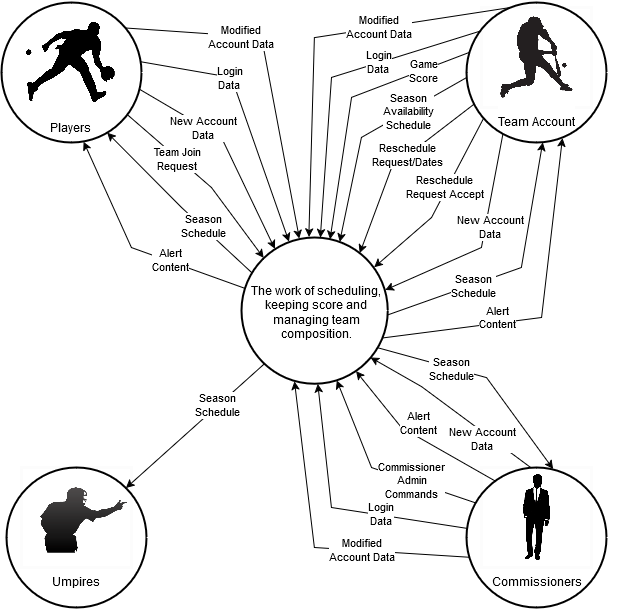
\includegraphics[scale=0.6]{6_2_context_diagram.png}
\subsection{Work Partitioning}
  \begin{center}
    \begin{tabular}{|m{4cm}|m{4cm}|m{6cm}|}
      \hline
      Event Name & Input and Output & Summary of BUC\\
      \hline
      1. User creates an account & New Account Data (in) & A player, team account, or
      commissioner enters in a username and password along with account details
      including their name, email, phone number, and gender.\\
      2. User logs in & Login Data (in) & A player, team account, or commissioner
      enters their username and password and the system grants them access to
      their account.\\
      3. Team account is created & New Team Information (in) & At the
      start of the season, a user can enter team information such as a team
      name. This registers a new team.\\
      4. Player requests to join a team & Team Join Request (in) & At the
      start of the season, players are not assigned to a team and must request
      to join one.\\
      5. Season starts and availability entered & Season Availability Schedule
      (in) & Record the team captain's entered availability schedule. This
      will be used to generate the league schedule.\\
      6. Reschedule request entered & Reschedule Dates (in) & Record
      availability dates the requesting captain entered as alternates for the
      planned date.\\
      7. Reschedule request received & Reschedule Dates (out) & Send the dates
      the captain who sent the request submit to the other team's captain.\\
      8. User navigates to schedule section & Season Schedule (out) & Display
      stored season schedule (if available) to site user.\\
      9. User navigates to contact information & Contact Infromation (out) & Display
      stored contact information (requires specific access) to site user.\\
      10. User submits alert & Alert Content (in) & Commissioners can submit custom
      alerts to send to any chosen users.\\
      \hline
    \end{tabular}
  \end{center}

  \begin{center}
    \begin{tabular}{|m{4cm}|m{4cm}|m{6cm}|}
      \hline
      11. System sends alert & Alert Content (out) & Send the alert to any user the
      alert must reach.\\
      12. Commissioner inputs admin command & Commissioner Admin Commands (in)
      & Commissioners have the ability to overwrite team composition and
      schedule.\\
      13. Captain submits game score & Game Score (in)
      & Captains submit the scores of games they have played into the
      system.\\
      14. User modifies account data & Account Password (if required) (in) \newline
      New Account Data (in) 
      & A player, team account, or commissioner modifies their account data (including account deletion)\\
      \hline
    \end{tabular}
  \end{center}

\subsection{Specifying a Business Use Case (BUC)}
Not applicable, events are simple and described in the work partitioning table
above.

\subsection{User Type Hierarchy}
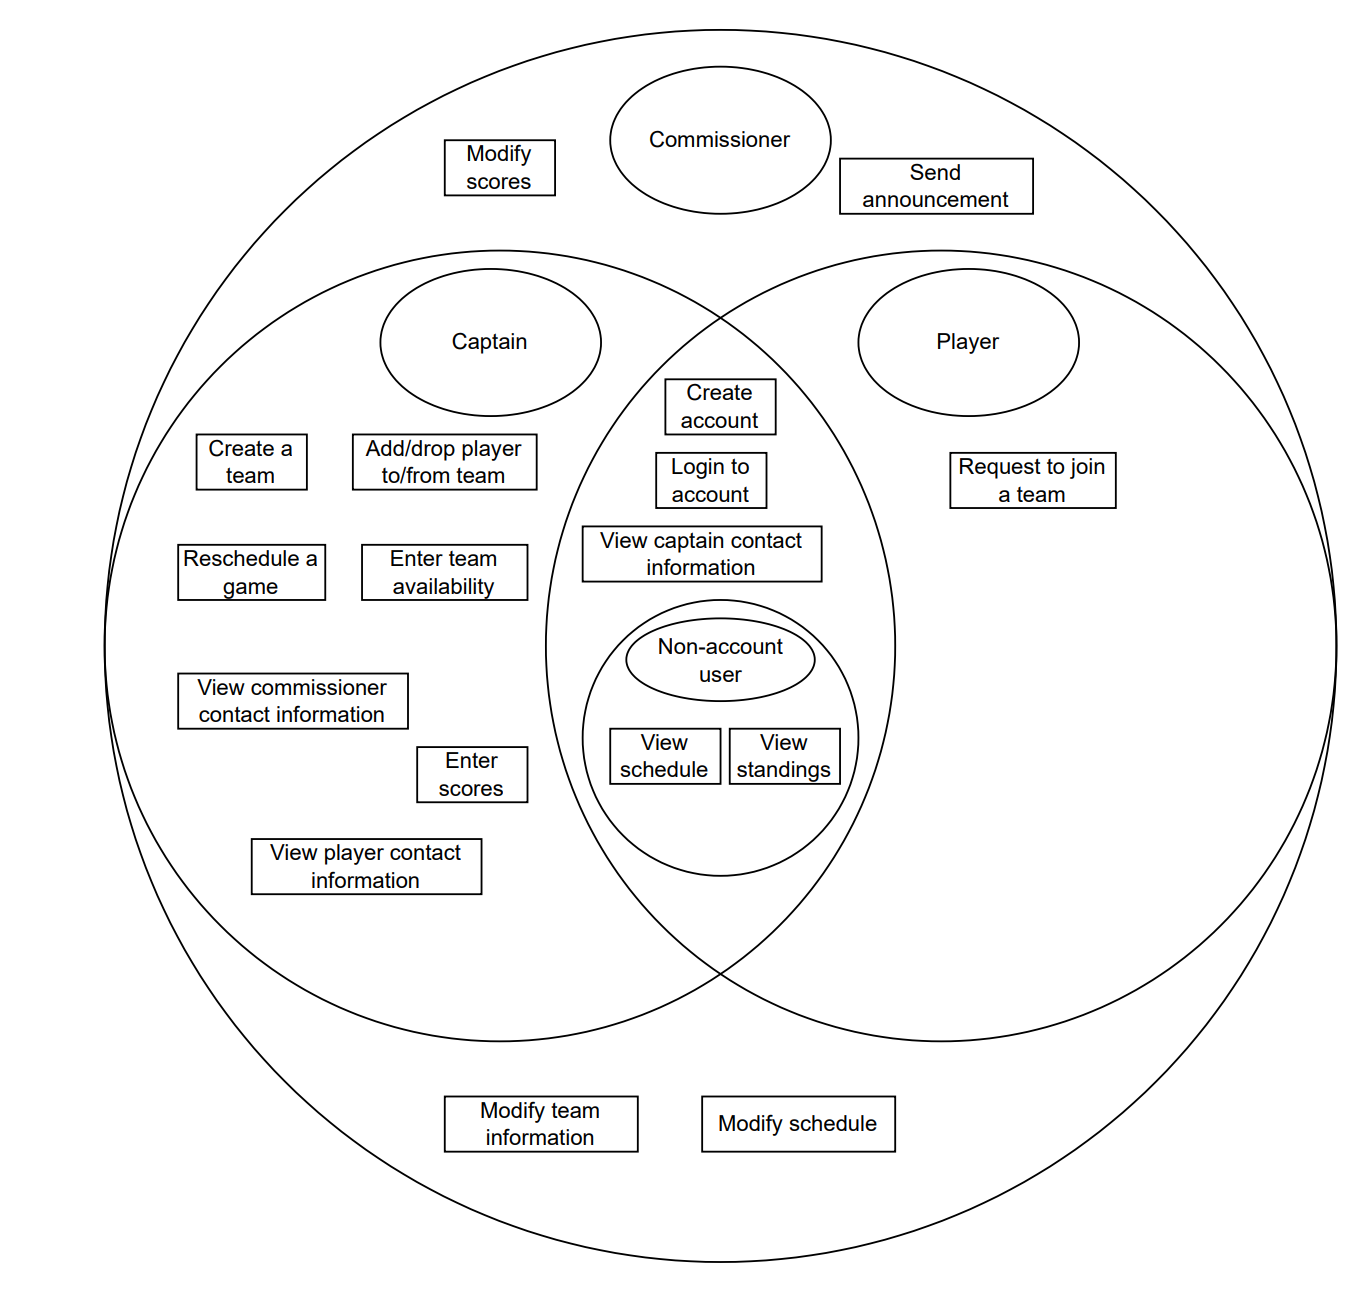
\includegraphics[scale=1.0]{business_data_model.png}

\section{Business Data Model and Data Dictionary}
\subsection{Business Data Model}
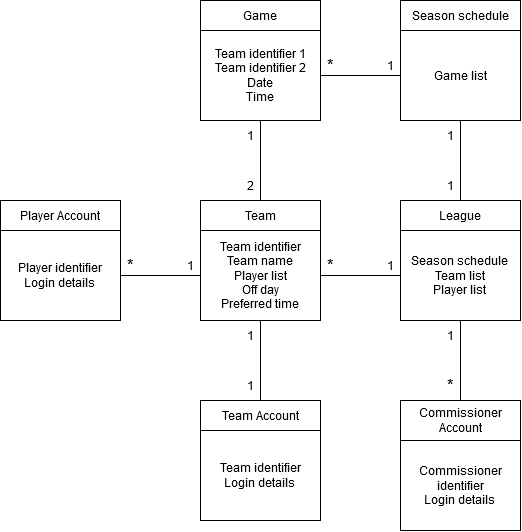
\includegraphics[scale=0.8]{7_1_business_diagram.png}

\subsection{Data Dictionary}
\begin{center}
  \begin{tabular}{|m{3cm}|m{8cm}|m{2cm}|}
    \hline
    Name & Content & Type\\
    \hline
    Player Account & Player identifier + Login details & Class\\
    \hline
    Team Account & Team identifier + Login details & Class\\
    \hline
    Commissioner Account & Commissioner identifier + Login details & Class\\
    \hline
    Team & Team identifier + Team name + Player list + Off day + Preferred
    time & Class\\
    \hline
    League & Season schedule + Team name + Player list & Class\\
    \hline
    Season schedule & {Game} & Class\\
    \hline
    Game & Team identifier + Team identifier + Date + Time & Class\\
    \hline
    Date & *YY/MM/DD* & Attribute\\
    \hline
    Time & *HH/MM/SS 24 hour clock*& Attribute\\
    \hline
    Player identifier & *Integer between 1 and 10 000* & Attribute\\
    \hline
    Team identifier & *Integer between 1 and 1000* & Attribute\\
    \hline
    Login details & *User defined username and password*& Attribute\\
    \hline
    Commissioner identifier & *Same as Player identifier* & Attribute\\
    \hline
    Player list & *List of player identifiers* & Attribute\\
    \hline
    Team list & *List of team identifiers* & Attribute\\
    \hline
  \end{tabular}
\end{center}

\section{The Scope of the Product}
Not applicable, content of this section is covered in Section 6.
\subsection{Product Boundary}
Not applicable.
\subsection{Product Use Case Table}
Not applicable.
\subsection{Individual Product Use Cases (PUC's)}
Not applicable.

\section{Functional Requirements}
\subsection{Functional Requirements}

\begin{myreq}
  \twoinline
    {\reqno FR-1}
    {\reqevent 7}
  \reqdesc System must display the season schedule and standings.
  \reqrat Schedule and standings are important information to be displayed for the league.
  \reqorig Alex Verity
  \reqfit The schedule and standings shall be viewable.
  \twoinline
    {\reqsatis 4}
    {\reqdissat 4}
\end{myreq}

\begin{myreq}
  \twoinline
    {\reqno FR-2}
    {\reqevent 3}
  \reqdesc Captains should be able to create a team which is added to the
  Sandlot database.
  \reqrat Teams are defined by captains, in charge of scheduling and
  recording scores. Captains must be able to define teams at the start of the
  season.
  \reqorig Alex Verity
  \reqfit When captains make a team, it should be added to the Sandlot
  database.
  \twoinline
    {\reqsatis 3}
    {\reqdissat 3}
\end{myreq}

\begin{myreq}
  \twoinline
    {\reqno FR-3}
    {\reqevent 1}
  \reqdesc Users should be able to create a new account by providing 
  the necessary information pertaining to their type of account.
  \reqrat An account structure is necessary to be able to change 
  what a user of the system can see/do based on who they are. 
  For example, a player and captain should not be able to see/do 
  the same things or 2 players from different teams should not be 
  able to see/do the same things.
  \reqorig Casra Ghazanfari
  \reqfit When a user provides the necessary information 
  (for players this can include name, email, password, waiver;
  for team accounts this can include team name, preferred days/times of play,
  preferred division), 
  an account should be created from that information
  \twoinline
    {\reqsatis 3}
    {\reqdissat 3}
\end{myreq}

\begin{myreq}
  \twoinline
    {\reqno FR-4}
    {\reqevent 14}
  \reqdesc Users should be able to change their account information 
  by providing the necessary information.
  \reqrat User information does not stay the same forever, 
  therefore the system should have a way for the user to change 
  their information if it ever changes.
  \reqorig Casra Ghazanfari
  \reqfit When a user provides the necessary information, 
  their account information should change.
  \twoinline
    {\reqsatis 3}
    {\reqdissat 4}
\end{myreq}

\begin{myreq}
  \twoinline
    {\reqno FR-5}
    {\reqevent 14}
  \reqdesc Users should be able to delete their account by providing 
  the necessary information.
  \reqrat If a user wants to quit the league they should be able to
  delete any of their personal information at any time.
  \reqorig Casra Ghazanfari
  \reqfit When a user provides the necessary information, 
  their account should be deleted.
  \twoinline
    {\reqsatis 3}
    {\reqdissat 2}
\end{myreq}

\begin{myreq}
  \twoinline
    {\reqno FR-6}
    {\reqevent 8,9}
  \reqdesc Commissioners should be able to send alerts with custom information
  to a specified user or group of users.
  \reqrat Commissioners have the need to notify league members with any new
  information relevant to the league. 
  \reqorig Alex Verity
  \reqfit When a commissioner enters information to alert league members, the
  league members receive a notification with the relevant information.
  \twoinline
    {\reqsatis 2}
    {\reqdissat 2}
\end{myreq}

\begin{myreq}
  \twoinline
    {\reqno FR-7}
    {\reqevent 9}
  \reqdesc Commissioners should be able to update the team information of any
  team, including player list and scores.
  \reqrat Commissioners have the need to easily fix any errors made by users.
  \reqorig Alex Verity
  \reqfit When a commissioner enters team information to be changed, the
  changes are made in the database.
  \twoinline
    {\reqsatis 3}
    {\reqdissat 3}
\end{myreq}

\begin{myreq}
  \twoinline
    {\reqno FR-8}
    {\reqevent 3}
  \reqdesc Before the season starts, captains must have the option to give
  their team's availability for the season.
  \reqrat Each team will have members who may only be free on certain days of
  the season. This availability will inform the season schedule so that teams
  will have as many people attending each game as possible.
  \reqorig Alex Verity
  \reqfit Before the season starts, captains shall be able to view the option to
  enter their availability and once entered, it shall be stored by the system
  to be used for scheduling.
  \twoinline
    {\reqsatis 4}
    {\reqdissat 4}
\end{myreq}

\begin{myreq}
  \twoinline
    {\reqno FR-9}
    {\reqevent 3}
  \reqdesc Once the season start due date is reached, all captain's
  availability will be used to generate a season schedule.
  \reqrat Once the season starts all users need to know the schedule to know
  when and where to go to games.
  \reqorig Alex Verity
  \reqfit When the season start due date is reached, a season schedule shall
  be displayed on the website.
  \twoinline
    {\reqsatis 2}
    {\reqdissat 3}
\end{myreq}

\begin{myreq}
  \twoinline
    {\reqno FR-10}
    {\reqevent 6}
  \reqdesc Captains must be able to request a rescheduling for their team's
  upcoming games as long as the game is at least 24 hours in the future.
  Rescheduling involves giving a list of alternate dates which are sent to
  the opposing team's captain to choose a date and accept.
  \reqrat Rescheduling is a core feature of the product, and schedule changes
  less than a day from when they are to occur may be too little warning for
  players to prepare for.
  \reqorig Alex Verity
  \reqfit A captain shall have the option to request rescheduling for games
  only more than RESCHED\_NOTICE\_HRS hours in the future.
  \twoinline
    {\reqsatis 5}
    {\reqdissat 5}
\end{myreq}

\begin{myreq}
  \twoinline
    {\reqno FR-11}
    {\reqevent 3}
  \reqdesc When a captain receives a rescheduling request, the system should
  prompt the captain to either accept the request and choose a date
  from the list of alternate dates, or deny the request.
  \reqrat Sometimes a captain may not be able to reschedule a game due to
  prior commitments or some other external factors. Therefore, there should be
  both an option to accept or deny any resheduling request.
  \reqorig Casra Ghazanfari
  \reqfit A captain shall have the option to either accept or deny any request
  to reschedule a game.
  \twoinline
    {\reqsatis 5}
    {\reqdissat 5}
\end{myreq}

\begin{myreq}
  \twoinline
    {\reqno FR-12}
    {\reqevent 3}
  \reqdesc When a captain's rescheduling request is either accepted or denied the
  system should notify them about the outcome.
  \reqrat It is important that the sender of the rescheduling request is informed
  about the status of the request quickly
  \reqorig Casra Ghazanfari
  \reqfit A captain who sent a rescheduling request shall be notified on the
  status of the request when it is responded to. 
  \twoinline
    {\reqsatis 4}
    {\reqdissat 4}
\end{myreq}

\begin{myreq}
  \twoinline
    {\reqno FR-13}
    {\reqevent 9}
  \reqdesc Captains should be able to update their team name and player list.
  \reqrat Captains are representatives of their teams and should have the ability
  to control information about their team on a high level. However, they should not
  have the same power as the commissioner and therefore should only be able to change 
  information related to their team.
  \reqorig Casra Ghazanfari
  \reqfit A captain shall have the ability to update team information.
  \twoinline
    {\reqsatis 4}
    {\reqdissat 4}
\end{myreq}

\begin{myreq}
  \twoinline
    {\reqno FR-14}
    {\reqevent 13}
  \reqdesc Captains should be able to submit scores for a game their team has
  played after the game has been completed.
  \reqrat Once a game is completed the system must know what the score was to
  accurately keep track of standings. The most reliable way to achieve this is
  a captain submitting it.
  \reqorig Nicholas Fabugais-Inaba
  \reqfit The captain should be able to submit a score after their scheduled
  game time is passed.
  \twoinline
    {\reqsatis 2}
    {\reqdissat 3}
\end{myreq}

\begin{myreq}
  \twoinline
    {\reqno FR-15}
    {\reqevent 4}
  \reqdesc Players should be able to join a team.
  \reqrat Players need to join a team to get a team schedule and play in the
  league.
  \reqorig Nicholas Fabugais-Inaba
  \reqfit When a player joins a team they are added to the team's player list.
  \twoinline
    {\reqsatis 4}
    {\reqdissat 5}
\end{myreq}

\begin{myreq}
  \twoinline
    {\reqno FR-16}
    {\reqevent 2}
  \reqdesc Account holders should be able to log in to Sandlot.
  \reqrat After a user makes an account they will need to access that account
  to use account related features.
  \reqorig Alex Verity
  \reqfit When a player enters valid account data the solution logs them in to
  their account.
  \twoinline
    {\reqsatis 5}
    {\reqdissat 5}
\end{myreq}

\begin{myreq}
  \reqno FR-17
  \reqdesc If the season start availability due date hasn't been reached, a
  captain should be able to resubmit availability data which overwrites
  previous availability data.
  \reqrat If the captain makes an error when submitting availability data
  they should be able to fix their error.
  \reqorig Alex Verity
  \reqfit If the captain has submitted data, they shall be able to overwrite
  it with new data.
  \twoinline
    {\reqsatis 4}
    {\reqdissat 4}
\end{myreq}

\begin{myreq}
  \reqno FR-18
  \reqdesc Commissioners should be able to edit the league schedule.
  \reqrat Commissioners have admin level permissions and should be able to
  modify the schedule to account for unforeseen problems.
  \reqorig Alex Verity
  \reqfit If the commissioner inputs new schedule data, the schedule
  reflects the updates made.
  \twoinline
    {\reqsatis 3}
    {\reqdissat 3}
\end{myreq}

\begin{myreq}
  \reqno FR-19
  \reqdesc Commissioners are able to assign captain level permissions to
  users.
  \reqrat Commissioners should be able to assign captains as captains are 
  needed to create and manage teams.
  \reqorig Alex Verity
  \reqfit If the commissioner assigns a user to captain, the user's account
  will gain captain level permissions.
  \twoinline
    {\reqsatis 4}
    {\reqdissat 4}
\end{myreq}

\begin{myreq}
  \reqno FR-20
  \reqdesc The system must display a schedule that includes all past and
  future games from all teams on a calendar.
  \reqrat All users need to know the league's schedule.
  \reqorig Jung Woo Lee
  \reqfit The system shall display a schedule that includes all past and
  future games from all teams on a calendar.
  \twoinline
    {\reqsatis 4}
    {\reqdissat 3}
\end{myreq}

\begin{myreq}
  \reqno FR-21
  \reqdesc The system must display a team schedule for each team that includes
  all the team's past and future games.
  \reqrat Users would like to see an individual team's schedule.
  \reqorig Jung Woo Lee
  \reqfit For each team, the system shall display a schedule that includes all
  past and future games from the team.
  \twoinline
    {\reqsatis 4}
    {\reqdissat 3}
\end{myreq}

\begin{myreq}
  \reqno FR-22
  \reqdesc The system must display a schedule that displays all upcoming games
  within a short time interval specified by the commissioner from the present.
  \reqrat Users would like to see a schedule focused on the soonest games in
  the season.
  \reqorig Jung Woo Lee
  \reqfit The system shall display a schedule that displays all upcoming games
  within a short time interval specified by the commissioner from the present.
  \twoinline
    {\reqsatis 4}
    {\reqdissat 3}
\end{myreq}

\begin{myreq}
  \reqno FR-23
  \reqdesc There can be only one captain associated with each team. Players
  who are captains of other teams do not count towards the one captain limit.
  \reqrat Based on the league rules, teams are only allowed one captain.
  \reqorig Jung Woo Lee
  \reqfit No team can have more than one captain associated with the team.
  \twoinline
    {\reqsatis 3}
    {\reqdissat 3}
\end{myreq}

\begin{myreq}
  \reqno FR-24
  \reqdesc The system must require the user to sign the league's waiver when
  they are creating a new account.
  \reqrat Based on the league's legal requirements, a player must sign a
  waiver to participate in the league.
  \reqorig Nicholas Fabugais-Inaba
  \reqfit The waiver form is signed by the user when they are creating an
  account.
  \twoinline
    {\reqsatis 4}
    {\reqdissat 4}
\end{myreq}

\section{Look and Feel Requirements}
\subsection{Appearance Requirements}

\begin{myreq}
  \reqno AP-1
  \reqdesc All user input elements should be distinctive such that they can be
  contrasted. 
  \reqrat User input should be clear to all users so users know where to enter
  inputs.
  \reqorig Alex Verity
  \reqfit User input elements shall have a minimum width and length of
  MIN\_INPUT\_SIZE pixels, maintain at least a MIN\_CONTRAST\_RATIO contrast
  ratio with the background.
  \twoinline
    {\reqsatis 2}
    {\reqdissat 4}
\end{myreq}

\begin{myreq}
  \reqno AP-2
  \reqdesc All user input elements should provide feedback.
  \reqrat Users should be able to know if their inputs are working or not.
  \reqorig Alex Verity
  \reqfit User input elements shall include distinct visual feedback (e.g.,
  color change or shadow) on hover or click for clear visibility and
  interactivity.
  \twoinline
    {\reqsatis 2}
    {\reqdissat 4}
\end{myreq}

\begin{myreq}
  \reqno AP-3
  \reqdesc All images and visuals made for/by Sandlot should be high quality.
  \reqrat Low quality images and visuals are unprofessional, and the solution
  should appear professional when possible. Only images made for/by Sandlot
  are included in this requirement as older photos or other visuals may need
  to be displayed that don't meet this standard.
  \reqorig Alex Verity
  \reqfit All images made for/by Sandlot shall be free of pixelation or
  blurring at their displayed size.
  \twoinline
    {\reqsatis 2}
    {\reqdissat 2}
\end{myreq}

\begin{myreq}
  \reqno AP-4
  \reqdesc Navigation should be straightforward, with menus and links easily
  accessible and readable.
  \reqrat Users should know what section of the site they will be accessing
  when they click on a navigation option so they don't get lost or confused.
  \reqorig Alex Verity
  \reqfit Navigation options shall be placed across all pages and their
  destination should be visibly written.
  \twoinline
    {\reqsatis 2}
    {\reqdissat 4}
\end{myreq}

\subsection{Style Requirements}

\begin{myreq}
  \reqno STY-1
  \reqdesc The solution should use the same colours, fonts and buttons across
  the entire user interface.
  \reqrat To ensure the professionalism of the solution, the style should
  feel unified and consistent to all users.
  \reqorig Alex Verity
  \reqfit All interface elements shall use fonts, colors and user input fields
  that are the same as those used in another section of the solution, ensuring
  a cohesive visual style and branding.
  \twoinline
    {\reqsatis 2}
    {\reqdissat 2}
\end{myreq}

\section{Usability and Humanity Requirements}
\subsection{Ease of Use Requirements}

\begin{myreq}
  \twoinline
    {\reqno EU-1}
    {\reqevent 7}
  \reqdesc Users must be able to easily find the season schedule.
  \reqrat Many users of Sandlot will not be using it often, and the
  schedule will be one of the most frequented parts of Sandlot. It must be
  easy to find and access. 
  \reqorig Alex Verity
  \reqfit On average, a new user shall not take more than one minute to find
  the schedule, and it should not take more than MAX\_NAV\_CLICKS clicks to
  access.
  \twoinline
    {\reqsatis 3}
    {\reqdissat 5}
\end{myreq}

\begin{myreq}
  \reqno EU-2
  \reqdesc Misinputted user login information shall provide a warning to the
  user, if login information does not exist or does not match the database
  stored login information.
  \reqrat Login information stored in the database should match the user
  inputted login information. Feedback should be provided for the user to
  understand an error has occurred when accessing an account with incorrect
  login details.
  \reqorig Nicholas Fabugais-Inaba
  \reqfit Assuming the user has misinputted the login details for
  an account stored in the database, they should be given a warning that
  notifies them about the login information being incorrect or not existing
  in the database.
  \twoinline
    {\reqsatis 3}
    {\reqdissat 5}
\end{myreq}

\begin{myreq}
  \reqno EU-3
  \reqdesc Teams will be given a warning if their availability data has
  scheduling conflicts.
  \reqrat The system should be able to create a valid schedule, in which
  teams do not have conflicting availability data that schedules games for
  the same dates and times as other teams.
  \reqorig Nicholas Fabugais-Inaba
  \reqfit Teams should receive a warning about their availability data
  conflicting on the schedule.
  \twoinline
    {\reqsatis 3}
    {\reqdissat 5}
\end{myreq}

\subsection{Personalization and Internationalization Requirements}
Not applicable.

\subsection{Learning Requirements}

\begin{myreq}
  \twoinline
    {\reqno LR-1}
    {\reqevent 7}
  \reqdesc A commissioner should be able to learn how to perform all of
  their available actions in a short amount of time.
  \reqrat Commissioners will need to make the necessary changes to the 
  product as the league plays out or changes season, and they have the most
  available actions that need to be learned.
  \reqorig Jung Woo Lee
  \reqfit A new commissioner to the product should be able to learn all of
  their possible actions within MAX\_TRAIN\_MINS minutes.
  \twoinline
    {\reqsatis 3}
    {\reqdissat 2}
\end{myreq}

\begin{myreq}
  \twoinline
    {\reqno LR-2}
    {\reqevent 7}
  \reqdesc A captain should be able to learn how to perform all of
  their available actions in a short amount of time.
  \reqrat Captains have certain actions that will be available to them that
  require some learning
  \reqorig Jung Woo Lee
  \reqfit A new captain to the product should be able to learn all of their
  possible actions within MAX\_TRAIN\_MINS minutes.
  \twoinline
    {\reqsatis 3}
    {\reqdissat 2}
\end{myreq}

\begin{myreq}
  \twoinline
    {\reqno LR-3}
    {\reqevent 7}
  \reqdesc A new user should be able to use the basic features (such as
  viewing the league schedule) of the product without having prior knowledge
  of the product.
  \reqrat All users should be able to intuitively perform some actions such as 
  viewing the season schedule.
  \reqorig Jung Woo Lee
  \reqfit A new user should be able to navigate to the season schedule on
  their first time interacting with the product.
  \twoinline
    {\reqsatis 3}
    {\reqdissat 2}
\end{myreq}

\subsection{Understandability and Politeness Requirements}

\begin{myreq}
  \reqno UP-1
  \reqdesc Any terminology or symbols used are the same as ones used in the
  past solution.
  \reqrat The terminology used should be the same as the past solution to
  make sure there is little confusion. For example the term off day will be
  used during scheduling as that is used in the past solution.
  \reqorig Alex Verity
  \reqfit MIN\_UNDERSTAND\_PERCENT percent of users understand terminology
  used on the Sandlot user interface.
  \twoinline
    {\reqsatis 3}
    {\reqdissat 2}
\end{myreq}

\subsection{Accessibility Requirements}

\begin{myreq}
  \reqno AC-1
  \reqdesc The fonts used should be readable by all users.
  \reqrat Sandlot will have a wide variety of users, and we must make sure the
  font is an appropriate size for those with reduced vision.
  \reqorig Alex Verity
  \reqfit Body text shall have a minimum font size of MIN\_FONT\_SIZE pixels,
  and a line length between MIN\_LINE\_CHARS characters and MAX\_LINE\_CHARS
  characters for optimal readability across all devices.
  \twoinline
    {\reqsatis 3}
    {\reqdissat 4}
\end{myreq}

\begin{myreq}
  \reqno AC-2
  \reqdesc Colours used should be colour blind friendly.
  \reqrat Sandlot will have a wide variety of users, and we must make sure the
  colours can be contrasted by all users.
  \reqorig Jung Woo Lee
  \reqfit  All colours applied to elements users will interact with must have
  a contrast ratio of at least MIN\_CONTRAST\_RATIO.
  \twoinline
    {\reqsatis 2}
    {\reqdissat 4}
\end{myreq}

\begin{myreq}
  \reqno AC-3
  \reqdesc Alerts sent to users must be visible and readable.
  \reqrat User may travel to a game that was postponed or cancelled, or miss
  out on critical information.
  \reqorig Nicholas Fabugais-Inaba
  \reqfit User receives an alert that is readable and clear enough for them
  to understand.
  \twoinline
    {\reqsatis 2}
    {\reqdissat 3}
\end{myreq}

\section{Performance Requirements}
\subsection{Speed and Latency Requirements}

\begin{myreq}
  \reqno SL-1
  \reqdesc Solution must load quickly and provide smooth user interactions,
  ensuring minimal delays when accessing content.
  \reqrat Sandlot will need to be a solution users are not frustrated by to
  encourage use, and long load times are frustrating.
  \reqorig Alex Verity
  \reqfit The website shall load in under MAX\_LOAD\_SECS seconds on a stable
  internet connection.
  \twoinline
    {\reqsatis 2}
    {\reqdissat 5}
\end{myreq}

\subsection{Safety-Critical Requirements}
Not applicable.
\subsection{Precision or Accuracy Requirements}
Not applicable.
\subsection{Reliability and Availability}

\begin{myreq}
  \reqno RA-1
  \reqdesc All features of the solution will achieve 99 percent uptime.
  \reqrat The past solution often has features that will break and go down,
  such as the standings feature, which at the time of writing is down. Our
  solution should not have these uptime issues.
  \reqorig Alex Verity
  \reqfit All features of the solution shall be usable and visible
  MIN\_UPTIME\_PERCENT percent of the time.
  \twoinline
    {\reqsatis 2}
    {\reqdissat 4}
\end{myreq}

\subsection{Robustness or Fault-Tolerance Requirements}

Not applicable.

\subsection{Capacity Requirements}

\begin{myreq}
  \reqno CR-1
  \reqdesc Sandlot should function for upwards of 60 teams and 1500 players in
  the system at once.
  \reqrat Sandlot should be able to function even if the league increases in
  population between seasons.
  \reqorig Alex Verity
  \reqfit No faults should occur when MAX\_TEAMS teams with MAX\_TEAM\_PLAYERS
  players each are entered into the system.
  \twoinline
    {\reqsatis 2}
    {\reqdissat 2}
\end{myreq}

\begin{myreq}
  \reqno CR-2
  \reqdesc Sandlot should function for upwards of 500 concurrent users.
  \reqrat Sandlot should be able to function even if a large portion of the
  league including spectators are using the solution.
  \reqorig Alex Verity
  \reqfit No faults should occur when MAX\_USERS users are using the system at
  once.
  \twoinline
    {\reqsatis 3}
    {\reqdissat 3}
\end{myreq}

\subsection{Scalability or Extensibility Requirements}
Not applicable.
\subsection{Longevity Requirements}
Not applicable.

\section{Operational and Environmental Requirements}
\subsection{Expected Physical Environment}
Not applicable.
\subsection{Wider Environment Requirements}
Not applicable.
\subsection{Requirements for Interfacing with Adjacent Systems}

\begin{myreq}
  \reqno IAS-1
  \reqdesc Sandlot should function on the last four releases for the five
  most popular browsers.
  \reqrat Sandlot should be accessible to a wide variety of users.
  \reqorig Alex Verity
  \reqfit The site shall function on the last four releases for the five most
  popular browsers.
  \twoinline
    {\reqsatis 2}
    {\reqdissat 4}
\end{myreq}

\subsection{Productization Requirements}
Not applicable.
\subsection{Release Requirements}

\begin{myreq}
  \reqno RR-1
  \reqdesc Sandlot will be released between league seasons.
  \reqrat Data will be difficult to transfer to Sandlot mid-season, Sandlot
  will not have that functionality on release.
  \reqorig Alex Verity
  \reqfit The solution shall be released between league seasons.
  \twoinline
    {\reqsatis 2}
    {\reqdissat 2}
\end{myreq}

\section{Maintainability and Support Requirements}
\subsection{Maintenance Requirements}

\begin{myreq}
  \reqno MR-1
  \reqdesc A new season can be started (i.e. saving past standings, resetting
  teams.) within one hour.
  \reqrat New seasons should not require a lot of maintenance to reset.
  \reqorig Alex Verity
  \reqfit A new season can be started within MAX\_SEASON\_START\_HRS.
  \twoinline
    {\reqsatis 5}
    {\reqdissat 5}
\end{myreq}

\subsection{Supportability Requirements}
Not applicable, however commissioners will support users if they can.

\subsection{Adaptability Requirements}
Not applicable, our solution will run on the web.

\section{Security Requirements}
\subsection{Access Requirements}

\begin{myreq}
  \reqno AS-1
  \reqdesc Viewing the league schedule and standings are accessible by any
  users of the system, logged in or not.
  \reqrat Viewing the schedule or standings should be accessible by spectators
  and umpires who will not have accounts in the system.
  \reqorig Jung Woo Lee
  \reqfit The league schedule and standings should be visible to all users
  including those not logged in.
  \twoinline
    {\reqsatis 5}
    {\reqdissat 5}
\end{myreq}

\begin{myreq}
  \twoinline
    {\reqno AS-2}
    {\reqevent 9}
  \reqdesc Players can only see the contact information of their own captain.
  \reqrat Players may need to contact their captain but should not have
  access to every account's information.
  \reqorig Nicholas Fabugais-Inaba
  \reqfit Players shall not be able to see any contact information outside
  their team's captain.
  \twoinline
    {\reqsatis 2}
    {\reqdissat 2}
\end{myreq}

\begin{myreq}
  \twoinline
    {\reqno AS-3}
    {\reqevent 9}
  \reqdesc Captains can only see the contact information of players on their
  own team and other team captains.
  \reqrat Captains may need to contact their players and other team captains
  but should not have access to every account's information.
  \reqorig Nicholas Fabugais-Inaba
  \reqfit Captains shall not be able to see any contact information outside of
  players on their team or other team captains.
  \twoinline
    {\reqsatis 2}
    {\reqdissat 2}
\end{myreq}

\begin{myreq}
  \twoinline
    {\reqno AS-4}
    {\reqevent 9}
  \reqdesc Commissioners can see the contact information of everyone in the
  league.
  \reqrat Commissioners may need to contact any account in the system.
  \reqorig Nicholas Fabugais-Inaba
  \reqfit Commissioners shall be able to see any account's contact
  information.
  \twoinline
    {\reqsatis 3}
    {\reqdissat 3}
\end{myreq}

\begin{myreq}
  \reqno AS-5
  \reqdesc Giving permissions to users must be accompanied by a warning that
  warns the user of the severity of the action.
  \reqrat Accidentally giving permissions to users who should not have them
  could result in unexpected errors.
  \reqorig Alex Verity
  \reqfit If permissions are being changed, a warning shall be displayed to
  the user before updating the permissions.
  \twoinline
    {\reqsatis 3}
    {\reqdissat 2}
\end{myreq}

\begin{myreq}
  \reqno AS-6
  \reqdesc Users can only access an account with correctly inputted login
  information that matches the database stored login information.
  \reqrat Login information stored in the database should correspond to a
  specific account. The account should only be accessed by the correctly
  inputted login information details.
  \reqorig Nicholas Fabugais-Inaba
  \reqfit Assuming the user has correctly inputted the login details for
  an account stored in the database, they should be granted access into
  the corresponding account.
  \twoinline
    {\reqsatis 3}
    {\reqdissat 3}
\end{myreq}

\begin{myreq}
  \reqno AS-7
  \reqdesc Captains can join a team that they are not the captain of.
  \reqrat Captains should be able to join a team they are not a part of, the
  league allows players to be on multiple teams.
  \reqorig Jung Woo Lee
  \reqfit If a captain attempts to join a team they are not the captain of,
  they will be added to the player list of the team.
  \twoinline
    {\reqsatis 2}
    {\reqdissat 5}
\end{myreq}

\begin{myreq}
  \reqno AS-8
  \reqdesc If a captain is a member of a team they are not the captain of,
  they only have player level permissions relating to that team.
  \reqrat Captains should not have captain permissions for any teams other
  than the team that they are the captain of.
  \reqorig Alex Verity
  \reqfit A captain can only do actions available to a player in a team that
  is not their own.
  \twoinline
    {\reqsatis 3}
    {\reqdissat 3}
\end{myreq}

\begin{myreq}
  \reqno AS-9
  \reqdesc Only commissioners can assign teams to a division.
  \reqrat Users not logged in as a commissioner should not be able to assign
  teams to a division.
  \reqorig Nicholas Fabugais-Inaba
  \reqfit Commissioners are able to assign a team to a division.
  \twoinline
    {\reqsatis 3}
    {\reqdissat 3}
\end{myreq}

\subsection{Integrity Requirements}

\begin{myreq}
  \twoinline
    {\reqno IG-1}
    {\reqevent 5}
  \reqdesc Website must not create conflicts when scheduling games.
  \reqrat The system shall create a schedule for all the teams in the league,
  without scheduling conflicts. Rescheduled games must also not conflict with the
  season schedule.
  \reqorig Nicholas Fabugais-Inaba
  \reqfit There exists no conflicts in the season schedule when the season begins or
  throughout the season when games are rescheduled.
  \twoinline
    {\reqsatis 4}
    {\reqdissat 4}
\end{myreq}

\begin{myreq}
  \reqno IG-2
  \reqdesc If there is only one commissioner level account, that account
  cannot be deleted.
  \reqrat Deleting this account would stop any more commissioner level
  accounts from being created, soft-locking the system.
  \reqorig Alex Verity
  \reqfit If there is only one commissioner level account it shall not be
  deleted.
  \twoinline
    {\reqsatis 3}
    {\reqdissat 3}
\end{myreq}


\begin{myreq}
  \reqno IG-3
  \reqdesc All match scores must be visible and contestable by other
  captains once recorded.
  \reqrat Match score correctness is extremely important for a competitive
  league, if a score is wrong, captains should be able to request that it be
  fixed.
  \reqorig Alex Verity
  \reqfit Any match scores shall have the option to be viewed and contested
  by captains.
  \twoinline
    {\reqsatis 4}
    {\reqdissat 4}
\end{myreq}

\begin{myreq}
  \reqno IG-4
  \reqdesc Captains are adequately notified when they receive an alert or a
  rescheduling request.
  \reqrat Important information may be shared in alerts, and reschedule
  requests that go unanswered may be frustrating for captains. Notifications
  should reach their intended targets if possible.
  \reqorig Alex Verity
  \reqfit Assuming the user hasn't interfered, alerts and reschedule requests
  shall always be sent to a place the user receives notifications.
  \twoinline
    {\reqsatis 4}
    {\reqdissat 4}
\end{myreq}

\subsection{Privacy Requirements}

\begin{myreq}
  \twoinline
    {\reqno PV-1}
    {\reqevent 1}
  \reqdesc The product shall not reveal contact information to any
  parties without the necessary access.
  \reqrat Contact information must be kept private within the league.
  \reqorig Nicholas Fabugais-Inaba
  \reqfit Contact information cannot be accessed by users that do not have
  an account registered in the league.
  \twoinline
    {\reqsatis 5}
    {\reqdissat 5}
\end{myreq}

\begin{myreq}
  \reqno PV-2
  \reqdesc Users are reminded to keep their passwords secure.
  \reqrat If a user accesses another user's account they may do actions
  without the account owner's permission or that the account owner is unaware
  of.
  \reqorig Alex Verity
  \reqfit A reminder telling users to keep their passwords secret and secure
  is displayed to the user.
  \twoinline
    {\reqsatis 1}
    {\reqdissat 1}
\end{myreq}

\subsection{Audit Requirements}
Not applicable.
\subsection{Immunity Requirements}
Not applicable.

\section{Cultural Requirements}
\subsection{Cultural Requirements}

\begin{myreq}
  \twoinline
    {\reqno CL-1}
    {\reqevent 1}
  \reqdesc The product shall provide an option to not specify gender.
  \reqrat Users may not associate themselves as male or female.
  \reqorig Nicholas Fabugais-Inaba
  \reqfit A user must be able to choose an option to not specify their
  gender.
  \twoinline
    {\reqsatis 5}
    {\reqdissat 5} 
\end{myreq}

\section{Compliance Requirements}
\subsection{Legal Requirements}
Not applicable.
\subsection{Standards Compliance Requirements}
Not applicable.

\section{Open Issues}

\begin{itemize}

  \item There are no open issues

\end{itemize}

\section{Off-the-Shelf Solutions}
\subsection{Ready-Made Products}
Not applicable.
\subsection{Reusable Components}
Not applicable.
\subsection{Products That Can Be Copied}
Not applicable.

\section{New Problems}
\subsection{Effects on the Current Environment}
Not applicable.
\subsection{Effects on the Installed Systems}
Not applicable.
\subsection{Potential User Problems}

Existing users of the current platform may suffer from the migration
to the new platform as they may not be familiar with how to navigate
the new system and utilize certain functions/features. This could be
concerning considering the age group and lack of technical literacy
for some users. One precaution that can be taken is to create a user
guide to aid users in interacting with the new system and the various
features it has to offer.

\subsection{Limitations in the Anticipated Implementation Environment That May
Inhibit the New Product}
Not applicable.
\subsection{Follow-Up Problems}
Not applicable.

\section{Tasks}
\subsection{Project Planning}

Within each requirement definition, the Customer Satisfaction rating details the
priority, in which, the requirement should be completed. Once high priority
functional requirements are complete, high priority non-functional requirements
will come next. These priorities are detailed below: \\\\

High-Functional: Customer Satisfaction Rating (5-4)

High-Non-Functional: Customer Satisfaction Rating (5-4)

Low-Functional: Customer Satisfaction Rating (3-1)

Low-Non-Functional: Customer Satisfaction Rating (3-1)

\subsection{Planning of the Development Phases}

The planning of the development phases will proceed as follows, provided the time
constraints and current project deadlines: \\\\
Critical requirements will be initially addressed with lower priority requirements
being investigated in the future. \\\\

Proof of Concept Demonstration (November 11-22):
\begin{itemize}
  \item Authentication: AS-13 and EU-2
  \item Scheduling: FR-17, AC-1, AC-2, and EU-3
\end{itemize}

Rev0 Demonstration (Revision 0) (February 3-14):
\begin{itemize}
  \item All high priority (see section 21.1 above) requirements are met.
\end{itemize}

Final Demonstration (Revision 1) (March 24-30):
\begin{itemize}
  \item All requirements, high and low priority, are met.
\end{itemize}

\section{Migration to the New Product}
\subsection{Requirements for Migration to the New Product}
Not applicable, we plan to begin use of Sandlot between seasons so that
current season data does not need to be transferred between systems aside from
archived past season standings.

\subsection{Data That Has to be Modified or Translated for the New System}

\begin{myreq}
  \reqno DMT-1
  \reqdesc There will exist an archive of past seasons that displays past
  season standings and results.
  \reqrat Users may be disappointed if new solution overwrites past season
  achievements.
  \reqorig Alex Verity
  \reqfit Past season standings shall be viewable on Sandlot.
  \twoinline
    {\reqsatis 1}
    {\reqdissat 2}
\end{myreq}

\section{Costs}
Not applicable.
\section{User Documentation and Training}
\subsection{User Documentation Requirements}

\begin{myreq}
  \reqno UD-1
  \reqdesc There must exist a user guide that informs users of the previous
  system and new users how to make an account, request to join a team, create
  a team, add players to the team, enter team availability, enter scores and
  reschedule a game.
  \reqrat There will be many new users of the system who might not be familiar
  with how to use the features of our solution, and will require guidance.
  \reqorig Alex Verity
  \reqfit There shall exist a user guide that explains all major features of
  the system.
  \twoinline
    {\reqsatis 3}
    {\reqdissat 1}
\end{myreq}

\subsection{Training Requirements}
Not applicable.

\section{Waiting Room}
Not applicable.

\section{Ideas for Solution}
Not applicable.

\newpage{}
\section*{Appendix --- Reflection}

The information in this section will be used to evaluate the team members on the
graduate attribute of Lifelong Learning.  Please answer the following questions:

\subsection*{Team -- Reflection}

\begin{enumerate}
  \item What knowledge and skills will the team collectively need to acquire to
  successfully complete this capstone project?  Examples of possible knowledge
  to acquire include domain specific knowledge from the domain of your
  application, or software engineering knowledge, mechatronics knowledge or
  computer science knowledge.  Skills may be related to technology, or writing,
  or presentation, or team management, etc.  You should look to identify at
  least one item for each team member.

  The team collectively needs to acquire lots of knowledge skills to successfully 
  complete this capstone project. In particular, Web development skills and knowledge 
  about the React language  will be key in developing a working website efficiently. SQL 
  skills and knowledge about database design and data migrations will be extremely useful 
  when working to store the website’s information properly. Knowledge on hosting these 
  different pieces of the project as well as learning how to properly integrate our project 
  with the host and finally, domain knowledge of the UI/UX design of existing scheduling 
  solutions on the market so that we can learn from existing solutions to ensure our 
  ease-of-use and user experience is top of the line. Casra will take on the web development 
  skills and knowledge, Nicholas will tackle the SQL skills and database knowledge, 
  Alex will look into hosting information and integrations, and Jung Woo will look into 
  domain knowledge of existing scheduling systems.

  \item For each of the knowledge areas and skills identified in the previous
  question, what are at least two approaches to acquiring the knowledge or
  mastering the skill?  Of the identified approaches, which will each team
  member pursue, and why did they make this choice?

  Web development skills and knowledge of the React language can be learned either by reading 
  the React documentation or by starting a separate test project and spending some time 
  learning by experimenting with the language. SQL skills and database design knowledge can 
  be learned by either creating practice queries on a dummy database or taking an online 
  structured learning course. Knowledge about hosting the different components of the project 
  can be gained by getting hands-on experience with cloud hosting platforms such as Microsoft 
  Azure or AWS or by testing hosting in a local environment on our own computers. To gain 
  domain knowledge of UI/UX design of scheduling platforms can either be gained by 
  investigating existing systems hands on and analyzing their UI/UX or by surveying people 
  about different applications they use and what parts of them they like/dislike.
  Casra will pursue learning web development and React by creating a separate test project 
  because he finds that learning by doing is much more effective for him than other methods. 
  Nicholas will pursue learning SQL and database design by taking an structured online course 
  on the subject because he feels that the more structured nature of the course will help him 
  learn consistently. Alex will pursue getting hands-on experience with cloud hosting 
  platforms because these platforms are likely what we will be using for the project and 
  so getting experience with them would be beneficial. Finally, Jung Woo will pursue 
  investigating the UI/UX domain knowledge and design of existing scheduling systems hands 
  on because he feels as though he will learn more from the existing system will give 
  insights into the developer's perspective of UI/UX design which will be helpful for us as 
  the developers.

\end{enumerate}

\subsection*{Alex Verity -- Reflection}

\begin{enumerate}
  \item What went well while writing this deliverable?\\\\
  The parts that went well for me were the non-functional requirements, I felt
  the look and feel section gave me a much better idea of what the solution is
  going to look like. The TA meeting was also extremely helpful and gave me a
  much better perspective on the project and confidence in our solution.
  \item What pain points did you experience during this deliverable, and how
  did you resolve them?\\\\
  Some pain points experienced were trying to get full coverage when coming up
  with use cases and functional requirements, we have many more questions for
  the supervisor now and will almost certainly need to come back to this
  document and modify it with new information we receive. I still don't know
  if the use cases provided are well put together or not and will be looking
  heavily at feedback in that area.
  \item How many of your requirements were inspired by speaking to your
  client(s) or their proxies (e.g. your peers, stakeholders, potential users)?
  \\\\
  Almost all requirements are inspired by speaking to our supervisor and
  primary stakeholder, as he defined the entire project during meetings with
  him. We were also heavily inspired by the TA meeting, where many of the
  look and feel requirements and user guide requirements came from, as well
  as advice on what to make into functional requirements.
  \item Which of the courses you have taken, or are currently taking, will help
  your team to be successful with your capstone project.\\\\
  The class 4HC3, whose subject is human computer interfaces and talks mainly
  about designing user interface. One of the main goals of the project is
  designing the UI to be more readable and better designed than the current
  solution, so any learning in that regard will be vital.

\end{enumerate}

\subsection*{Jung Woo Lee -- Reflection}

\begin{enumerate}
  \item What went well while writing this deliverable?\\\\
  Coming up with most of the requirements was easier than expected due to the breadth of information we had from talking with the supervisor on the product.
  
  
  \item What pain points did you experience during this deliverable, and how
  did you resolve them?\\\\
  Going through and working on this document, made me realize how much more we as a team probably need to know about user needs. Sometimes we were left with questions on if something was a requirement or not. All of this indicated to the fact that we need to have more time to speak to our supervisor.
  
  \item How many of your requirements were inspired by speaking to your
  client(s) or their proxies (e.g. your peers, stakeholders, potential users)?\\\\
  Almost all of the requirements came from the supervisor, who is both a potential user and stakeholder. With the initial information he provided us on the problem and desired product, we could develop most of these requirements. A few of the requirements were not explicitly told to us, but could be inferred and others have been created by us to conform with ethical practices for example.
  
  \item Which of the courses you have taken, or are currently taking, will help
  your team to be successful with your capstone project.\\\\
  All project based courses are definitely useful to understand project dynamics. Dealing with a team, and performing to certain standards has been taught to us in all of these various courses. Providing deliverables and project scheduling has also been taught to us, such that administrative duties are easier for us to tackle. The databases course will likely help us as our project will most likely be using this in our solution. The user-interface course will help us in creating a human-centered design that is intuitive and clean. This is one of the pitfalls of the current solution, and thus one of the important non-functional requirements. The requirements course will also help us interpret requirements going forward and make use of our work here. And late it will undoubtedly help us revise this document.

\end{enumerate}

\subsection*{Nicholas Fabugais-Inaba -- Reflection}

\begin{enumerate}
  \item What went well while writing this deliverable?\\\\
  When writing this deliverable, outlining the different requirements associated
  with the varying aspects of the project helped in understanding what is required
  from the team to accomplish a completed product for this project. More specifically,
  outlining the access requirements and creating the hierarchy diagram aided in
  my understanding of how each user will interact with the system.
  \item What pain points did you experience during this deliverable, and how
  did you resolve them?\\\\
  Some of the pain points from this deliverable was the amount of content 
  needed to be covered with all of the different sections. With so many different
  types of requirements in mind and the number of overlapping requirements, it
  was incredibly difficult to fill in each section or understand why a certain
  type of requirement may not apply to the project. These pain points were resolved
  by brainstorming as a team our own requirements that we would then review
  amongst each other to understand if the requirement was satisfactory enough
  or if it should be constructed in a different way.
  \item How many of your requirements were inspired by speaking to your
  client(s) or their proxies (e.g. your peers, stakeholders, potential users)?
  \\\\
  From both the TA and the initial meeting with the project supervisor, the team
  was able to get a grasp on the requirements that must be important to mention
  in the SRS. Mainly the project supervisor was able to outline the overall
  requirements needed to improve on the existing system, however, the TA was 
  still able to provide valuable insight into either how general or how specific
  a requirement should be defined.
  \item Which of the courses you have taken, or are currently taking, will help
  your team to be successful with your capstone project.\\\\
  Specifically for the SRS, our software requirements class that is primarily taken
  in the 3rd year for software engineering students aided in the creation
  of the SRS document. Additionally, our software design III course will help the
  team be successful with the capstone project as we had created a prototype design
  similar to Uber. Collaborating with a team for a project that had many moving
  parts to it should surely aid in the creation of the team's initial MVP for
  the project as well as the development towards the final product that will
  be showcased early in 2025.

\end{enumerate}

\subsection*{Casra Ghazanfari -- Reflection}

\begin{enumerate}
  \item What went well while writing this deliverable?\\\\
  Writing the functional requirements section of this deliverable went well 
  because we had access to the old existing system that the project is aiming 
  to improve upon. This allowed us to look at the old existing system’s functionalities 
  and easily come up with functional requirements that the new system would need to meet 
  based on the old system’s functionalities.
  \item What pain points did you experience during this deliverable, and how
  did you resolve them?\\\\
  The biggest pain point during this deliverable was understanding what each section 
  of the document was asking for. Many sections of the document have unintuitive names 
  that do not accurately describe the information the section should hold. In addition, many 
  of the sections were either inapplicable or very loosely applicable to our project making 
  it difficult to understand which sections we should be tackling.
  \item How many of your requirements were inspired by speaking to your
  client(s) or their proxies (e.g. your peers, stakeholders, potential users)?
  \\\\
  There isn’t an exact number but ~25\% of our requirements are directly inspired/created 
  from information we got while talking to our client. Most prominently our look and feel 
  requirements were directly from our discussions where we learned that UX and ease of use 
  were extremely important factors for both the client and users of our system.
  \item Which of the courses you have taken, or are currently taking, will help
  your team to be successful with your capstone project.\\\\
  SFWRENG 3XB3 Software Engineering Practice and Experience is a project oriented software 
  design course which is, and will be extremely helpful for a successful capstone project. 
  3XB3 taught effective software design and got me used to the workflow of a software project 
  which will both be very applicable to our capstone.
\end{enumerate}

\end{document}